\documentclass{article}
\usepackage{amsmath}
\usepackage{amssymb}
\usepackage{ntheorem}
\usepackage{graphicx}
\usepackage{bbm}
\usepackage{hyperref}
\hypersetup{
	colorlinks=true,
	linkcolor=blue,
	filecolor=cyan,      
	urlcolor=red,
	citecolor=green,
}
\newtheorem{theorem}{Theorem}
\newtheorem{corollary}{Corollary}
\newtheorem{lemma}{Lemma}
\newtheorem*{proof}{Proof}
\setlength{\parindent}{2em}
\author{Siheng Zhang\\zhangsiheng@cvte.com}
\title{Chapter \textbf{\textit{4}} Linear Model}
\date{\today}
\usepackage[a4paper,left=18mm,right=18mm,top=25mm,bottom=25mm]{geometry} 

\begin{document}
\maketitle  

This part corresponds to \textbf{Chapter 1,3,4 of PRML, Chapter of UML}, and mainly answers the following questions:

\begin{itemize}
\item 
\end{itemize}

\tableofcontents
\newpage

\section{Linear classification}

	In the last chapter, we stops at the linear classification of binary classification task,
	
	\begin{equation}
	y=h(\mathbf{x})=\mathbf{w}^\top \mathbf{x} + w_0 = \sum_{j=1}^d w_j x_j + w_0
	\end{equation}
in which $\mathbf{w}$ is weight vector, and $w_0$ is bias. The input vector is assigned to class $C_1$ iff. $h(\mathbf{x})\geq 0$ and to class $C_2$ otherwise.

	Consider two points $\mathbf{x}_1,\mathbf{x}_2$ on the decision boundary, i.e., $\mathbf{w}^\top (\mathbf{x}_1 - \mathbf{x}_2) = 0$, hence $\mathbf{w}$ is orthogonal to the decision boundary. And the distance from the origin to the decision boundary is
	
	\begin{equation}
	\frac{\mathbf{w}^\top \mathbf{x}}{\|\mathbf{w}\|} = \frac{-w_0}{\|\mathbf{w}\|}
	\end{equation}
	
	It is usually convenient to use a more compact notation in which we introduce an additional input value $x_0 = 1$ and then define $\tilde{\mathbf{w}} = (w_0, \mathbf{w})$ and $\tilde{\mathbf{x}} = (x_0, \mathbf{x})$ so that $h(\mathbf{x}) = \tilde{\mathbf{w}}^\top \tilde{\mathbf{x}}$. For simplification, we neglect the `tilde' symbol below.
	
	\subsection{Extend to multiple classes}
	
	\begin{itemize}
	\item \textit{one-versus-the-rest} For each class $k=1,2,...,K$, each classifier judge whether an example is $C_k$ or not. So there are $K$ classifiers needed.
	\item \textit{one-versus-one} An alternative is to introduce $K(K-1)/2$ binary discriminant functions, one for every pair of classes (but will lead to ambiguous region).
	\end{itemize}
	
	\subsection{Fisher's linear discriminant}
	
	One way to view a linear classification model is in terms of dimensionality reduction. By adjusting the components of the weight vector $\mathbf{w}$, we can select a projection that maximizes the class separation. To begin with, consider a two-class problem in which there are $N_1$ points of class $C_1$ and $N_2$ points of class $C_2$, so that the mean vectors of the two classes are given by

	\begin{equation}
	\mathbf{m}_1 = \frac{1}{N_1} \sum_{\mathbf{x}_n \in C_1} \mathbf{x}_n,\ \ \ \ \ \ \ \ 
	\mathbf{m}_2 = \frac{1}{N_2} \sum_{\mathbf{x}_n \in C_2} \mathbf{x}_n
	\end{equation}
	
	The simplest measure of the separation of the classes, when projected onto $\mathbf{w}$, is the separation of the projected class means. This suggests that we might choose $w$ so as to maximize 
	\begin{equation}
	m_2- m_1=\mathbf{w}^\top (\mathbf{m}_2-\mathbf{m}_1)
	\end{equation}
where $m_k=\mathbf{w}^\top \mathbf{m}_k$ is the mean of the projected data from class $C_k$. 

	This expression can be made arbitrarily large simply by increasing the magnitude of $\mathbf{w}$. To solve this problem, we could constrain $\mathbf{w}$ to have unit length, i.e., $\|\mathbf{w}\|_2=1$. Using a Lagrange multiplier, it turns to maximize $\mathbf{w}^\top (\mathbf{m}_2-\mathbf{m}_1) + \lambda (1-\|\mathbf{w}\|_2)$, which leads to $\mathbf{w}\propto \mathbf{m}_2-\mathbf{m}_1$

\section{Linear regression}

	In linear regression model, the model is the same except that the learning target $y$ is continuous but not discrete. And the learning goal is the sum-of-square (SSE) loss

	\begin{equation}
	\min_\mathbf{w} L_S(h) = \sum_{i=1}^m (h(\mathbf{x}_i) - y_i)^2 = \sum_{i=1}^m (\mathbf{w}^\top\mathbf{x}_i - y_i)^2 
	\end{equation}

	Suppose the fitting error $\epsilon_i = y_i-\mathbf{wx}_i$ is Gaussian noise, i.e., $\epsilon_i \sim\mathcal{N}(0,\beta)$. Then the log likelihood function of the training sequence is
	
	\begin{equation}
	\log \mathcal{L} = -\frac{m}{2} \log 2\pi\beta - \sum_{i=1}^m \frac{(y_i-\mathbf{w}^\top\mathbf{x}_i)^2}{2\beta}
	\end{equation}

	Obviously, MLE is equivalent to linear regression.

	\textit{\underline{remark1}: Since linear regression is not a binary prediction task, we cannot analyse its sample complexity using the VC-dimension. One possible analysis of the sample complexity of linear regression is by relying on the "discretization trick". However, to apply the sample complexity bounds from Chapter 2 we also need that the loss function will be bounded.}
	
	\subsection{Generalized linear regression}
	
	The model is just a linear function of the input variables, and this imposes significant limitations on it. Therefore, extended model considers \textbf{linear} combination of fixed \textbf{non-linear} functions of the input variables, of the form
	
	\begin{equation}
	h(\mathbf{x}) = w_0 + \sum_{j=1}^d w_j \phi_j(x)
	\end{equation}
where $\phi_j(x)$ are known as \textit{basis functions}. Again, denote $\phi_0(\mathbf{x})=1$ so that $h(\mathbf{x}) = \tilde{\mathbf{w}}^\top \phi(\mathbf{x})$. For Simplification, we also neglect the `tilde' symbol from now on.

	Now, consider the closed-form solution for The gradient of the log likelihood. The gradient of the SSE loss takes the form
	
	\begin{equation*}
	\nabla L_S(h) = \sum_{i=1}^m \left\{ y_i - \mathbf{w}^\top \mathbf{\phi} (\mathbf{x}_i)) \right\} \mathbf{\phi}^\top (\mathbf{x}_i)
	\end{equation*}
Setting it to zero gives 

	\begin{equation}
	\label{eqn:mp_solved}
	\mathbf{w} = \mathbf{\Phi}^\dag \mathbf{y} = (\mathbf{\Phi}^\top \mathbf{\Phi})^{-1}\mathbf{\Phi}^\top \mathbf{y}
	\end{equation}
Here $\mathbf{\Phi}$ is an $n x d$ matrix, whose elements are given by $\mathbf{\Phi}_{nj} = \Phi_j(\mathbf{x}_n)$. And $\mathbf{\Phi}^\dag$ is \textit{Moore-Penrose pseudo-inverse}.

	\textit{\underline{remark2, multiple-outputs}: A more general case is multiple outputs, i.e., $\mathbf{y}_i \in \mathcal{R}^k, k>1$. However, the solution to multiple-outputs regression problem decouples between the different target variables so we do not discuss it here.}
	
	\textit{\underline{remark3, on-line learning}:} Batch techniques involve processing the entire training set in one go, can be computationally costly for large data sets. For linear regression, stochastic gradient descent algorithm updates parameter using
	
	\begin{equation*}
	\mathbf{w}^{t+1}=\mathbf{w}^{t} - lr*\nabla L_{(\mathbf{x}_t,y_t)}(h) = \mathbf{w}^{t} + lr* (y_i - (\mathbf{w}^t)^\top \mathbf{\phi} (\mathbf{x}_t)) \mathbf{\phi} (\mathbf{x}_t)
	\end{equation*}
in which $lr$ is the learning rate.

	\textit{\underline{remark3, basis}: There are three popular basis function: 1. \textbf{Polynomial basis}, 2. \textbf{Radical basis}, 3. \textbf{Fourier basis}.}
	
	\subsection{Regularization \textit{a.k.a} Bayesian linear regression}
	
	Recall the closed-form solution (Eq. \ref{eqn:mp_solved}) for linear regression problem, if $n\leq d$, the SSE loss can achieve zero. It means that the model capacity is enough for the training dataset. However, it may suffer from over-fitting problem. Consider the learning dataset generated from $y$.

\subsubsection{Ridge regression}

	Ridge regression addresses on over-fitting by penalizing the $l_2$-norm of weight vector $\mathbf{w}$,
	
	\begin{equation*}
	\min_\mathbf{w} \sum_{i=1}^m (\mathbf{w\phi_i(x)} - y_i)^2 + \lambda\|\mathbf{w}\|^2_2
	\end{equation*}

	If we assume a Gaussian prior for the weight vector, $\mathbf{w}\sim\mathcal{N}(0,\alpha^{-1}\mathbf{I})$, then the posterior of the training sequence is:
	
	\begin{equation}
	p(\mathbf{w}|S) \propto p(\mathbf{w}) p(S|\mathbf{w}) \propto \exp \left( -\frac{\alpha}{2} \mathbf{w}^\top \mathbf{w} \right) \cdot \prod_{i=1}^N \exp \left( -\frac{(y_i-\mathbf{wx}_i)^2}{2\beta} \right)
	\end{equation}
	
Maximizing the log posterior function is equivalent to the ridge regression.
	
	
\subsubsection{Lasso}

	Lasso addresses on over-fitting by penalizing the $l_1$-norm of weight vector $\mathbf{w}$,
		
	\begin{equation*}
	\min_\mathbf{w} \sum_{i=1}^m (\mathbf{w\phi_i(x)} - y_i)^2 + \lambda\|\mathbf{w}\|_1
	\end{equation*}
	
	If we assume a Laplace prior for the weight vector, $p(\mathbf{w})=\frac{1}{2\alpha} \exp \left( -\frac{\|\mathbf{w}\|_1}{\alpha} \right)$, then the posterior of the training sequence is:
	
	\begin{equation}
	p(\mathbf{w}|S) \propto p(\mathbf{w}) p(S|\mathbf{w}) \propto \exp \left( -\frac{\|\mathbf{w}\|_1}{\alpha} \right) \cdot \prod_{i=1}^N \exp \left( -\frac{(y_i-\mathbf{wx}_i)^2}{2\beta} \right)
	\end{equation}

Maximizing the log posterior function is equivalent to the Lasso model.

	\textit{\underline{remark2}: }
	\begin{figure}[!htbp]
	\begin{center}
	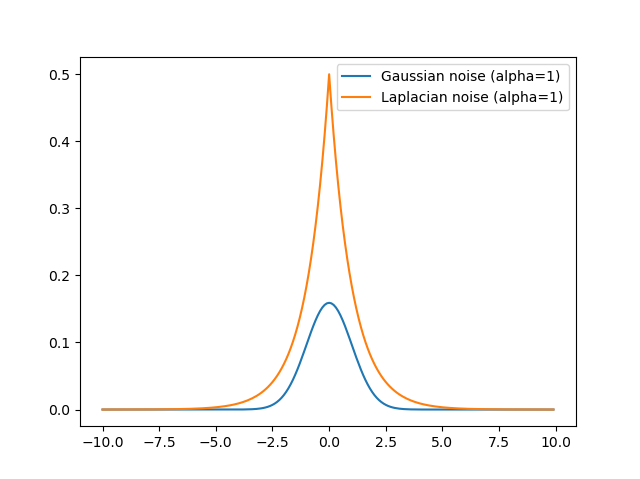
\includegraphics[scale=.4]{C4-1.png}	
	\end{center}
	\end{figure}

\end{document}